\documentclass[preprint, 3p,
authoryear]{elsarticle} %review=doublespace preprint=single 5p=2 column
%%% Begin My package additions %%%%%%%%%%%%%%%%%%%

\usepackage[hyphens]{url}

  \journal{Transport Geography?} % Sets Journal name

\usepackage{graphicx}
%%%%%%%%%%%%%%%% end my additions to header

\usepackage[T1]{fontenc}
\usepackage{lmodern}
\usepackage{amssymb,amsmath}
% TODO: Currently lineno needs to be loaded after amsmath because of conflict
% https://github.com/latex-lineno/lineno/issues/5
\usepackage{lineno} % add
\usepackage{ifxetex,ifluatex}
\usepackage{fixltx2e} % provides \textsubscript
% use upquote if available, for straight quotes in verbatim environments
\IfFileExists{upquote.sty}{\usepackage{upquote}}{}
\ifnum 0\ifxetex 1\fi\ifluatex 1\fi=0 % if pdftex
  \usepackage[utf8]{inputenc}
\else % if luatex or xelatex
  \usepackage{fontspec}
  \ifxetex
    \usepackage{xltxtra,xunicode}
  \fi
  \defaultfontfeatures{Mapping=tex-text,Scale=MatchLowercase}
  \newcommand{\euro}{€}
\fi
% use microtype if available
\IfFileExists{microtype.sty}{\usepackage{microtype}}{}
\usepackage[]{natbib}
\bibliographystyle{plainnat}

\usepackage{graphicx}
\ifxetex
  \usepackage[setpagesize=false, % page size defined by xetex
              unicode=false, % unicode breaks when used with xetex
              xetex]{hyperref}
\else
  \usepackage[unicode=true]{hyperref}
\fi
\hypersetup{breaklinks=true,
            bookmarks=true,
            pdfauthor={},
            pdftitle={Leveraging GTFS to explore spatial patterns in transit supply with respect to social needs},
            colorlinks=false,
            urlcolor=blue,
            linkcolor=magenta,
            pdfborder={0 0 0}}

\setcounter{secnumdepth}{5}
% Pandoc toggle for numbering sections (defaults to be off)


% tightlist command for lists without linebreak
\providecommand{\tightlist}{%
  \setlength{\itemsep}{0pt}\setlength{\parskip}{0pt}}




\usepackage{subfig}
\usepackage{booktabs}
\usepackage{longtable}
\usepackage{array}
\usepackage{multirow}
\usepackage{wrapfig}
\usepackage{float}
\usepackage{colortbl}
\usepackage{pdflscape}
\usepackage{tabu}
\usepackage{threeparttable}
\usepackage{threeparttablex}
\usepackage[normalem]{ulem}
\usepackage{makecell}
\usepackage{xcolor}



\begin{document}


\begin{frontmatter}

  \title{Leveraging GTFS to explore spatial patterns in transit supply
with respect to social needs}
    \author[Public Transport Research Group (PTRG)]{James Reynolds%
  %
  \fnref{1}}
   \ead{james.reynolds@monash.edu} 
    \author[Public Transport Research Group (PTRG)]{Graham Currie%
  \corref{cor1}%
  \fnref{2}}
   \ead{graham.currie@monash.edu} 
    \author[Public Transport Research Group (PTRG)]{Yanda Qu%
  %
  \fnref{3}}
   \ead{yanda.qu@monash.edu} 
      \affiliation[Public Transport Research Group (PTRG)]{
    organization={Public Transport Research Group (PTRG), Institute of
Transport Studies, Department of Civil Engineering Engineering, Monash
University},addressline={Clayton
Campus},city={Melbourne},postcode={3800},state={Victoria},country={Australia},}
    \cortext[cor1]{Corresponding author}
    \fntext[1]{Research Fellow}
    \fntext[2]{Professor}
    \fntext[3]{PhD Student}
  
  \begin{abstract}
  This is the abstract.

  It consists of two paragraphs.
  \end{abstract}
    \begin{keyword}
    keyword1 \sep 
    keyword2
  \end{keyword}
  
 \end{frontmatter}

\section{Introduction}\label{introduction}

Providing basic mobility for those who cannot otherwise drive is a key
purpose for transit in many places \citep{Currie:2016aa}. Age,
disability, socio-economic status, lack of a driver's license or
vehicle, and many other factors might make someone reliant on transit
services for some or all of their travel. Approaches for identifying
spatial gaps in transit supply,\\
where is a high or very high social need yet little or no service, have
been reported in previous research
\citep{Currie2003Hobart, Currie2004Gap, Currie2007Identifying, currie2010identifying}.

However, in the almost two decades since there does not appear to have
been much further use or development of these approach. As well, it is
unclear if the spatial patterns identified in this previous research are
representative of transit supply and social need in other places, or
whether the location of gaps have changed in the intervening years. This
may in part be because at the time transit schedule data was not readily
available in a consistent, electronic formats.

Nowadays, however, more than 10,000 transit agencies publicly release
schedule data in the General Transit Feed Specification (GTFS) format.
Various tools for manipulating such datasets are also now available,
including software for validating, analysing and visualizating GTFS, as
well as a separate standard (GTFS-Realtime) for sharing live vehicle
locations \citep{GTFS}.

However, software tools for examining spatial patterns and gaps in
transit supply with respect to social needs for transport appears
limited. This gap and the lack of direct follow up to
\citet{Currie2003Hobart}, \citet{Currie2004Gap},
\citet{Currie2007Identifying} and \citet{currie2010identifying} provide
the motivation for this paper. The three main objectives of the research
are: (1) to develop tools for undertaking needs-gap analysis using GTFS
datasets; (2) to explore whether such gaps have changed in the
intervening years; and (3) to better understand whether spatial patterns
in Melbourne are representative of those in other places.

This research included the development of a new R package
(gtfssupplyindex) with software tools that facilitate the use of the
\citet{Currie2003Hobart}, \citet{Currie2004Gap},
\citet{Currie2007Identifying} and \citet{currie2010identifying}
approach, in particular the calculation of transit Supply Index (SI)
scores from GTFS datasets. Also presented in this paper are results for
Australian cities in 2016 and 2021, matching the most recent censuses,
which are compared across locations and to the 2006 analysis of
Melbourne reported in \citet{currie2010identifying}.

The remainder of this paper is structured as follows: the next section
outlines the background to this research. Section 3 describes the study
methodology, followed by presentation of results in Section 4 and
discussion in Section 5. Limitations of this study, directions for
future research and a brief conclusion are provided in Section 6.

\section{Background}\label{background}

\subsection{Transit metrics}\label{transit-metrics}

There are many metrics available for benchmarking transit services,
including those in the Transit Cooperative Research Program (TCRP)
Report 88 guidebook on developing performance-measurement systems
\citep{Ryus:2003aa}; and those used across benchmarking databases and
programs (e.g. \citet{Florida-Transit-Information-System:2018aa},
\citet{UITP:2015aa} \citet{Imperial-College-London:2023aa}; The Fielding
Triangle \citep{FieldingGordonJ1987Mpts} provides a framework for
combining indicators of service inputs, outputs and consumption to
describe cost efficiency, cost effectiveness and service effectiveness.
More broadly: \citet{Litman:2003ab} and \citet{Litman:2016aa} discuss
some of the traffic, mobility, accessibility, social equity, strategic
planning and other rational decision-making-based perspectives underling
transport indicators; \citet{Reynolds:2017ah} extends these into models
of how institutionalism, incrementalism and other public policy analysis
concepts might apply to decision-making processes relating to transit
prioritization; \citet{GuzmanLuisA.2017Aeit} developed a measure of
accessibility in the context of policy development and social equity for
Latin American Bus Rapid Transit (BRT) networks; and
\citet{Creutzig2020streetspaceallocation} introduced street space
allocation metrics based around ten ethical principles.

However, many of these metrics may be difficult to calculate, explain or
understand, especially for those who are not planners, engineers or
other technical specialists. Where pre-calculated transit metrics are
immediately available, such as on a website or other online platform, it
may not be possible to independently generate scores, for instance to
assess proposed system changes. Contrasting examples are provided by the
metrics in the Transit Capacity and Quality of Service Manual (TCQSM)
and the Transit Score website \citep{WalkScore:2023tg}:

\begin{itemize}
\item
  Transit Scores are readily available online for locations with a
  published GTFS feed. The meaning of the metric also appears easy to
  explain, with the highest possible score of 100 representing the sort
  of transit accessibility experienced in the center of New York.
  However, the Transit Score algorithm is secret, and scores cannot be
  calculated independently or generated for proposed changes to
  networks.
\item
  The TCQSM provides a wide range of metrics for measuring different
  aspects of a transit system. The TCQSM scores themselves appear easy
  to understand or explain, ranging from A (good) to F (bad), although
  the large number of metrics might be somewhat overwhelming for some
  users. The scores, however, can be calculated independently, given
  sufficient data.
\end{itemize}

The widespread availability of GTFS datasets in recent years has
facilitated the development of tools, such as the Transit Score, that
apply the same metric to many transit systems. \citet{Wong:2013aa}
provides another example of what can be done with GTFS data, open
metrics and coding, by reporting the distribution of various TCQSM
metrics across 50 USA transit operators. Code used in the
\citet{Wong:2013aa} analysis is available for those who might wish to
produce a similar study for other locations and systems.

\subsection{The Transit Suppy Index}\label{the-transit-suppy-index}

An objective of this study is to produce code that facilitates
calculation of the SI metric from GTFS data. A generalized form of the
SI equation, adapted from \citet{currie2010identifying}, is:

\[SI_{area, time} = \sum{\frac{Area_{Bn}}{Area_{area}}*SL_{n, time}}\]

where:

\begin{itemize}
\item
  \(SI_{area, time}\) is the Supply Index for the area of interest and a
  given period of time;
\item
  \(Area_{Bn}\) is the buffer area for each stop (n) within the area of
  interest (in \citet{currie2010identifying} this was based on a radius
  of 400 metres for bus and tram stops, and 800 metres for railway
  stations);
\item
  \(Area_{area}\) is the area of the area of interest; and
\item
  \(SL_{n,time}\) is the number of transit arrivals for each stop for a
  given time period.
\end{itemize}

\begin{figure}
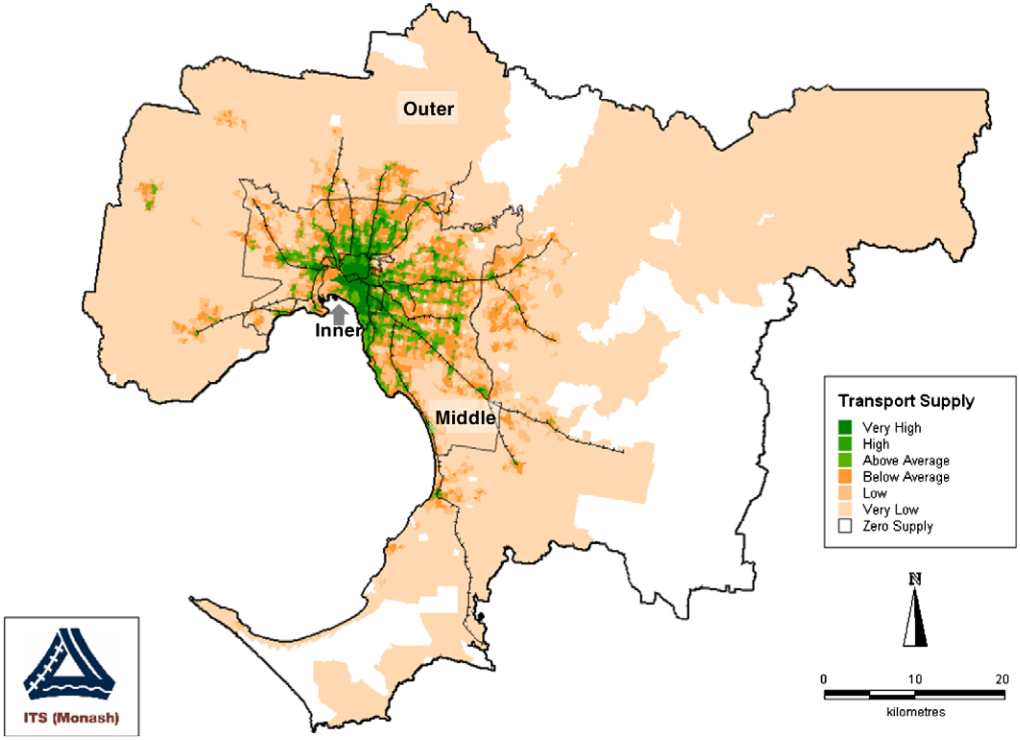
\includegraphics[width=1\linewidth]{graphics/Currie2010SI} \caption{Distribution of supply measure scores – Metropolitan Melbourne (2006), Source: Currie (2010)}\label{fig:Currie_map_SI}
\end{figure}

\citet{currie2010identifying} reported SI scores for Census Collection
Districts (CCDs) across Greater Melbourne in 2006, as shown in Figure
\ref{fig:Currie_map_SI}.\\
They identified general patterns of more transit supply in the middle
and inner suburbs and along passenger railway lines; and outer areas
tending to have very low SI scores or no transit supply at all.

\subsection{Social need and needs gap}\label{social-need-and-needs-gap}

\begin{figure}
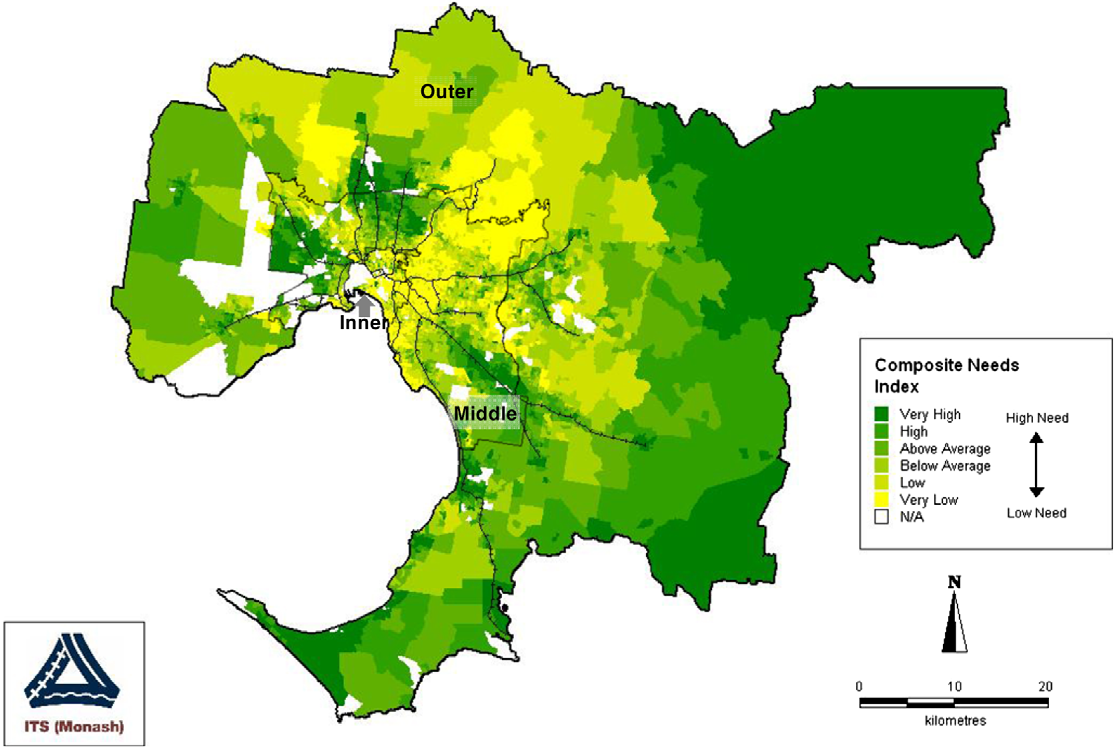
\includegraphics[width=1\linewidth]{graphics/Currie2010Needs} \caption{Distribution of categories of composite social need index scores in 2006, Source: Currie (2010)}\label{fig:Currie_map_needs}
\end{figure}

As well as measuring transit supply, \citet{currie2010identifying} also
assessed the social need for transit across Greater Melbourne using: the
Australian Bureaus of Statistics' Index of Related Socio-Economic
Advantage/Disadvantage (IRSAD) and a transport needs index derived from
eight weighted indicators. The spatial distribution of this composite
social needs index in 2006, reproduced in Figure
\textbackslash ref\{fig:Currie\_map\_needs), indicates areas of above
average, high and very high social needs in 2006 were located in: some
outer areas, particularly in the east and south-east; and in some middle
areas in the south-east, north and west.

\begin{figure}
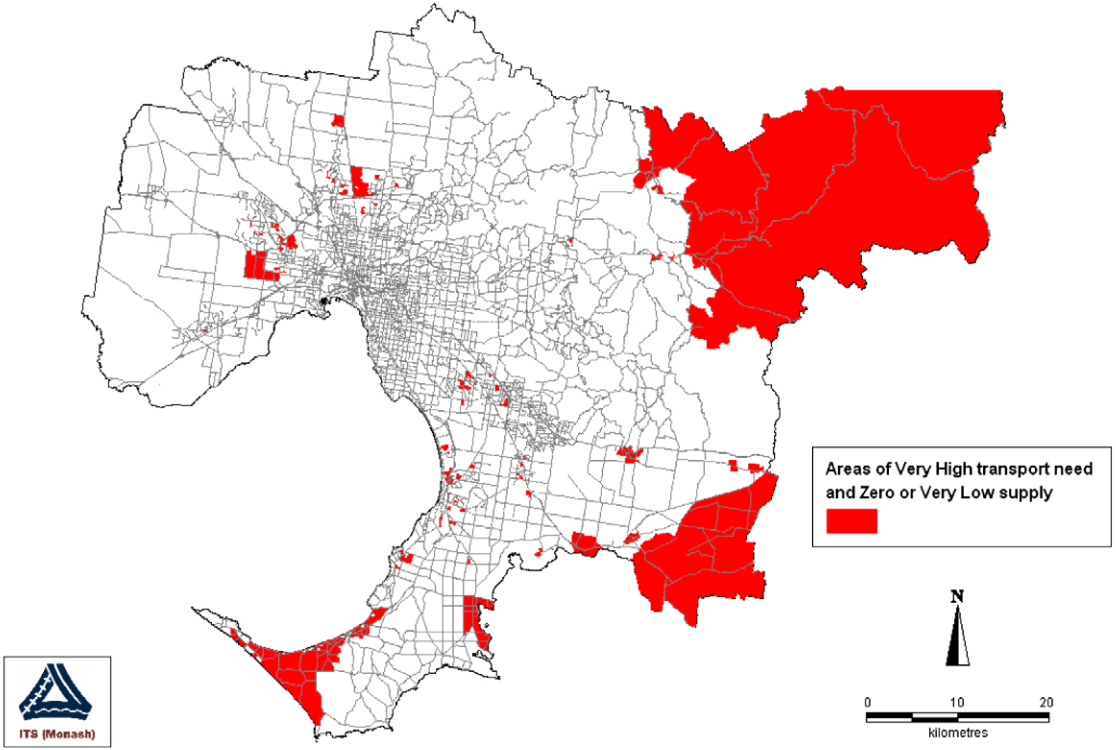
\includegraphics[width=1\linewidth]{graphics/Currie2010gap} \caption{Melbourne needs-gap in 2006 – very high transport need areas with zero or very low public transport supply, Source: Currie (2010)}\label{fig:Currie_map_gap}
\end{figure}

As the final step in the spatial needs-gap analysis,
\citet{currie2010identifying} identified areas with very high transport
needs, but very low or no transit supply,\\
as reproduced in Figure \ref{fig:Currie_map_gap}. This indicated areas
where service gaps might be of particular concern, Most of these were
located in outer parts of Melbourne in the north-east, south-east and
south, although there were also some pockets in the middle suburbs in
the west, north and south east. Overall, \citet{currie2010identifying}
found that ``8.2\% of Melbourne residents have `very high' needs but
`zero', `low' or `very low' public transport supply.'' Using this
methodology in transit planning was also suggested as ``substantially
more useful than the presentation of anecdotal evidence, which is the
most common means of identifying transport needs in local transport
studies throughout the world.''\citep{currie2010identifying}

However, it does not appear that this approach has been widely adopted
in practice or further developed by researchers. Our suspicion is that
while the SI has a relatively simple formula and requires only
geographic and timetable data, the lack of software tools may be partly
why it has not been more widely adopted.

It is also unclear whether the patterns in Melbourne identified in
\citet{currie2010identifying} have changed since the 2006 analysis, or
if Melbourne is representative of other locations. Developing a software
tool to calculate SI tools from GTFS data, and then using it to
comparing current conditions and other locations to the findings of
\citet{currie2010identifying}, therefore, provides the motivation for
this research.

\section{Methodology}\label{methodology}

\subsection{Code development}\label{code-development}

This study developed a package of tools for calculating the SI from GTFS
data using the R programming language \citep{R-base}. The
recommendations of \citet{wickham2023r} informed the package setup and
development approach. Various existing packages and code examples were
relied upon including: the sf package \citep{R-sf} for geospatial
analysis; the tidyverse \citep{tidyverse2019}; gtfstools
\citep{R-gtfstools}; and tidytransit \citep{R-tidytransit}. Australian
Bureau of Statistics (ABS) data was also used, sourced via the strayr
and absmapsdata packages \citep{r-strayr}.

Code was developed and tested on the Mornington Peninsula Tourist
Railway GTFS feed. This was selected primarily for convenience, given
that the authors are familiar with the surrounding geography and that
the feed covers a small number of trips across just three stations.

\subsection{Changes since 2006: Greater
Melbourne}\label{changes-since-2006-greater-melbourne}

Much has changed since 2006, including the spatial geography used by the
Australian Bureau of Statistics (ABS) to collect census data. To allow
direct comparison between 2006 and the most recent census, therefore,
this study calculated SI scores using the same Census Collection
Districts (CCDs) used by \citet{currie2010identifying} for the week
starting the day of the 2021 census The Victorian GTFS feed, published
by Public Transport Victoria (PTV), was used, with historical feeds
sourced via \citet{transitfeeds_victoria:2023aa}.

Unfortunately, it is not possible to obtain 2016 or 2021 social
disadvantage data for CCDs, as the ABS now releases data for SA zones
only. SA1 zones, therefore, are adopted for the comparison of social
needs-gaps in 2016 and 2021, as discussed in the following.

\subsection{Variation in spatial patterns across
location.}\label{variation-in-spatial-patterns-across-location.}

SI scores were also calculated for Greater Melbourne, Greater Brisbane,
Greater Perth, Greater Adelaide, Greater Hobart and the Australian
Capital Territory (which includes Canberra), again for the week starting
on the day of the 2021 census. Historical GTFS data was again sourced
via the Transit Feeds website, Unfortunately it was not possible to
locate historical GTFS data for Greater Sydney or Greater Darwin, so
instead the latest data sets were sourced directly from the relevant
transit authorities.

For comparison between cities, Statistical Area 1 (SA1) zones were
adopted from the Australian Bureau of Statistics \citep{ABSmaps} as the
areas of interest. This allowed direct comparison to ABS-reported values
for social and transport needs, population and other census data.

\subsection{Variation in time}\label{variation-in-time}

SHOULD THIS BE RUN FOR ALL YEARS AS FAR BACK AS THE GTFS DATA GOES??

\subsection{Measuring social
disadvantage}\label{measuring-social-disadvantage}

This study adopts a similar approach to measuring social disadvantage as
used in \citet{currie2010identifying}, using: the ABS' Index of Relative
Socio-Economic Advantage/Disadvantage (IRSAD); and a transport needs
index\footnote{The same need indicators and weightings used in
  \citet{currie2010identifying} were adopted, although \$799 or lower
  per week was used as the threshold for low income households rather
  than \$499 to account for inflation (as per Reserve Bank of
  Australia's online inflation calculator).}. A composite needs
indicator was derived based on the IRSAD and the transport needs index,
again as per the \citet{currie2010identifying} approach\footnote{However,
  changes to the ABS reporting systems mean that the composite needs
  indicator had to based on weighting both the IRSAD index and the
  transport need index by the total population of each SA1 zone, which
  were then added, standardised and split into six groups.}.

\section{Results}\label{results}

\subsection{The gtfssupplyindex
Package}\label{the-gtfssupplyindex-package}

Code developed to calculate SI scores is available as an R package on
github (see \citet{gtfssupplyindex_github}). Included in the package is
a vignette that outlines the structure of the calculations, the
developed functions (LINK HERE), and step-by-step calculations for the
Mornington Peninsula Railway as a worked example and comparison to SI
scores calculated manually.

\subsection{Greater Melbourne: changes since
2006}\label{greater-melbourne-changes-since-2006}

\subsubsection{2021 SI scores - CCDs}\label{si-scores---ccds}

\begin{figure}
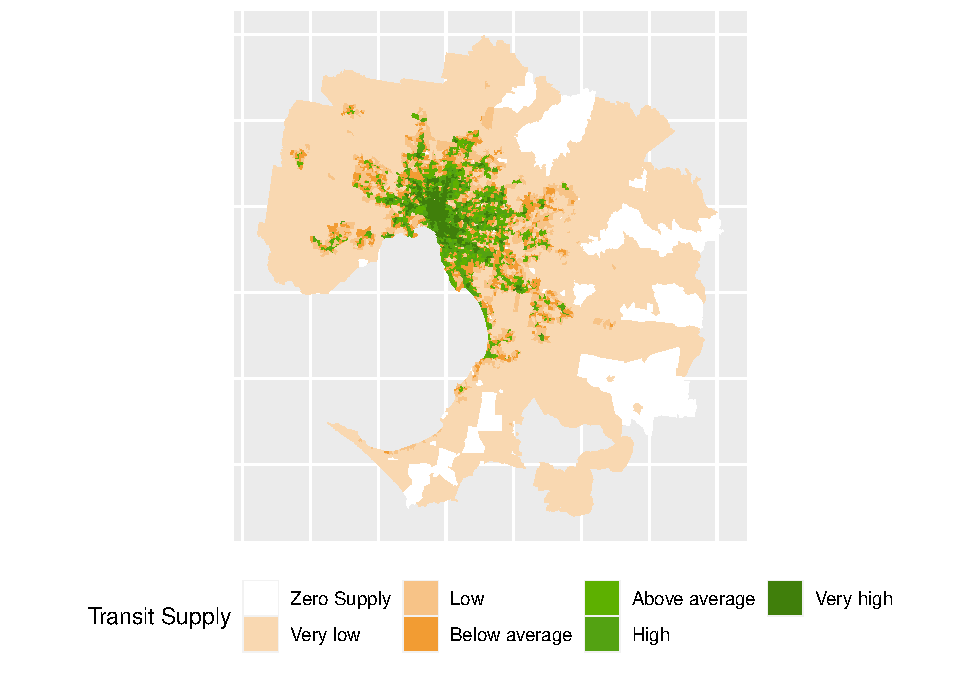
\includegraphics[width=1\linewidth]{Leveraging_GTFS_to_assess_transit_supply_Transport_Geography_files/figure-latex/Greater_Melbourne_CCD_2021-1} \caption{Greater Melbourne (2006 extents), Transport Supply by CCD, week starting the day of the 2021 census}\label{fig:Greater_Melbourne_CCD_2021}
\end{figure}

Figure \ref{fig:Greater_Melbourne_CCD_2021} shows SI scores for
Melbourne in the week of the 2021 census, using the same (2006) CCD
boundaries as in Figure \ref{fig:Currie_map_SI}. Comparing Figures
\ref{fig:Currie_map_SI} and \ref{fig:Greater_Melbourne_CCD_2021}
suggests that overall spatial patterns are generally similar in 2021 as
they were in 2006, with higher levels of transit supply in inner areas
and close to most railway lines. There are still many areas with very
low or zero transit supply, especially in outer areas. However, only 81
CCDs have Zero Supply in 2021, compared to the 186 reported in
\citet{currie2010identifying} for 2006. There are, however, slightly
more CCDs included in this 2021 analysis (6,326 compared to the 5,720 in
2006), meaning that the percentage of CCDs with Zero Supply has fallen
to 1.28\% from the 3.25\% in 2006. The average SI value has also
increased to 3,299.8 from its value of 2,886.9 in 2006, indicating that
the overall transit service supply score has increased by approximately
24\%.

\begin{figure}
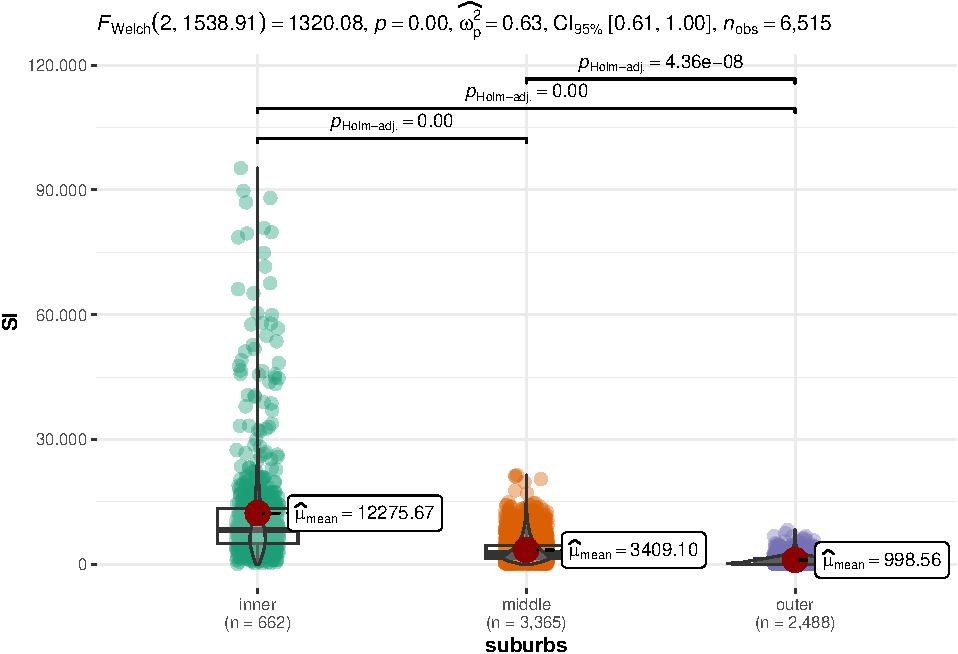
\includegraphics[width=1\linewidth]{Leveraging_GTFS_to_assess_transit_supply_Transport_Geography_files/figure-latex/Greater_Melbourne_CCD_2021_by_suburbs_SI_scores-1} \caption{Greater Melbourne (2006 extents), SI score by CCD, week starting the day of the 2021 census, inner, middle and outer suburbs}\label{fig:Greater_Melbourne_CCD_2021_by_suburbs_SI_scores}
\end{figure}

Figure \ref{fig:Greater_Melbourne_CCD_2021_by_suburbs_SI_scores}
compares 2021 SI scores for CCDs across the inner, middle and outer
suburbs. SI scores average 12,275.7, 3,409.1 and 998.6 for the inner,
middle and outer suburbs respectively\footnote{The same grouping of LGAs
  to inner, middle and outer suburb groups as used in
  \citet{currie2010identifying} was used for this analysis, although
  here the City of Stonnington was allocated entirely to the middle
  grouping, whereas \citet{currie2010identifying} allocated part of this
  LGA to the inner group.}. These compare to the scores of 10,922.7,
2,694.9 and 764.3, respectively, reported for 2006 in
\citet{currie2010identifying}.

\begin{table}

\caption{\label{tab:Greater_Melbourne_CCD_2021_by_suburbs}Distribtuion of CCDs by Transit Supply grouping across inner, middle and outer suburbs}
\centering
\begin{tabular}[t]{l|r|r|r|l}
\hline
transit\_supply & inner & middle & outer & Total\\
\hline
Zero Supply & 0.0\%   (0) & 8.6\%     (7) & 91.4\%    (74) & 100.0\%    (81)\\
\hline
Very Low & 0.7\%  (11) & 20.5\%   (303) & 78.8\% (1,166) & 100.0\% (1,480)\\
\hline
Low & 1.6\%  (24) & 47.1\%   (701) & 51.3\%   (764) & 100.0\% (1,489)\\
\hline
Below average & 3.7\%  (55) & 69.4\% (1,038) & 26.9\%   (402) & 100.0\% (1,495)\\
\hline
Above average & 8.8\%  (55) & 80.6\%   (506) & 10.7\%    (67) & 100.0\%   (628)\\
\hline
High & 21.9\% (146) & 76.0\%   (506) & 2.1\%    (14) & 100.0\%   (666)\\
\hline
Very High & 54.9\% (371) & 45.0\%   (304) & 0.1\%     (1) & 100.0\%   (676)\\
\hline
Total & 10.2\% (662) & 51.7\% (3,365) & 38.2\% (2,488) & 100.0\% (6,515)\\
\hline
\end{tabular}
\end{table}

\begin{figure}
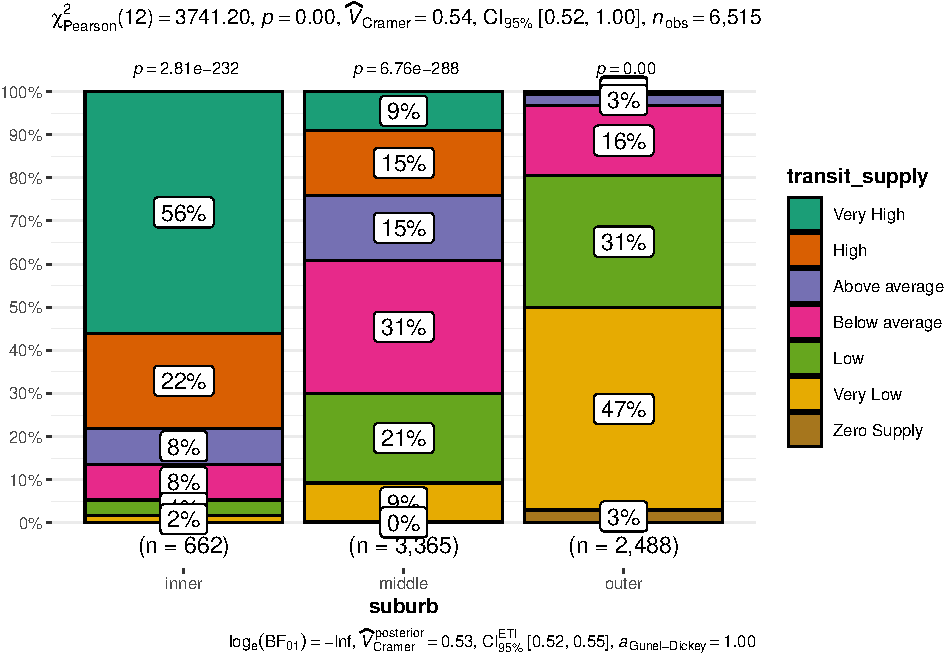
\includegraphics[width=1\linewidth]{Leveraging_GTFS_to_assess_transit_supply_Transport_Geography_files/figure-latex/Greater_Melbourne_CCD_2021_by_suburbs-1} \caption{Greater Melbourne (2006 extents), Distribution of CCDs by Transit Supply grouping, week starting the day of the 2021 census, for the inner, middle and outer suburbs}\label{fig:Greater_Melbourne_CCD_2021_by_suburbs}
\end{figure}

Table \ref{tab:Greater_Melbourne_CCD_2021_by_suburbs} and Figure
\ref{fig:Greater_Melbourne_CCD_2021_by_suburbs} compares the
distribution of Transport Supply groupings across the inner, middle and
outer suburbs. In general, the results meet expectations, with a greater
proportion of CCDs having higher transit supply in inner and (then)
middle suburbs.

\subsubsection{2021 SI scores - SA1s}\label{si-scores---sa1s}

The 2006 census was the last to use CCDs. Population and other data was
instead reported for SA1s in 2021, and Figure
\ref{fig:Greater_Melbourne_SA1_2021_plot} shows the 2021 Transit Supply
groupings using these zones. Greater Melbourne now covers a larger
spatial area, and so Figure \ref{fig:Greater_Melbourne_SA1_2021_plot}
shows includes all SA1 zones within the 2021 GCCSA boundary. The 2006
GCCSA boundary is also shown for comparison purposes. Table
\ref{tab:Greater_Melbourne_SA1_2021_table} and Figure
\ref{fig:Greater_Melbourne_SA1_2021_table} compare number of CCD and SA1
zones in each category in 2006 and 2021, as well as the share of Greater
Melbourne's population living in zones within each category.

\begin{figure}
\centering
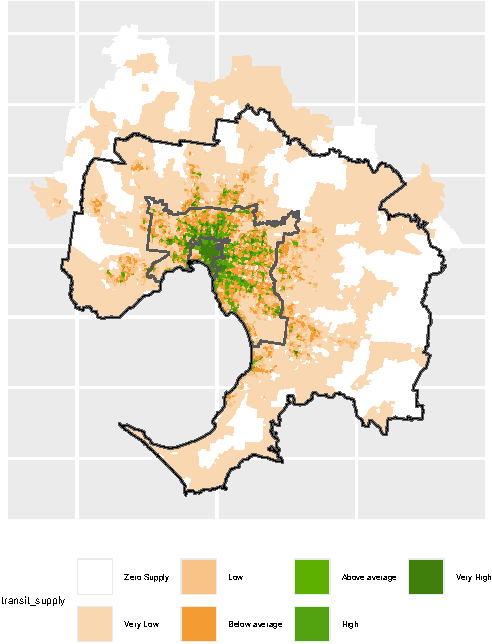
\includegraphics{Leveraging_GTFS_to_assess_transit_supply_Transport_Geography_files/figure-latex/Greater_Melbourne_SA1_2021_plot-1.pdf}
\caption{Greater Melbourne, Transit Supply by SA1, week starting the
date of 2021 census, with 2006 Melbourne boundary shown in black}
\end{figure}

\begin{table}

\caption{\label{tab:Greater_Melbourne_SA1_2021_table}Greater Melbourne: Distribution of supply index scores and resident population. Sources: 2006 values (Currie 2010), 2021 values (authors)}
\centering
\begin{tabular}[t]{l|r|r|r|r|r}
\hline
\multicolumn{1}{c|}{Supply Index} & \multicolumn{2}{c|}{CCDs} & \multicolumn{1}{c|}{SA1s} & \multicolumn{2}{c}{Population} \\
\cline{1-1} \cline{2-3} \cline{4-4} \cline{5-6}
category & 2006 & 2021 & 2021 & 2006 & 2021\\
\hline
Zero Supply & 3.2\%   (189) & 1.2\%    (81) & 4.3\%    (489) & 2.5\%    (85,423) & 3.8\%   (186,829)\\
\hline
Very Low & 22.5\% (1,314) & 22.7\% (1,480) & 23.4\%  (2,692) & 23.6\%   (793,046) & 23.0\% (1,132,967)\\
\hline
Low & 22.4\% (1,310) & 22.9\% (1,489) & 23.4\%  (2,691) & 25.7\%   (865,330) & 23.7\% (1,163,358)\\
\hline
Below average & 22.2\% (1,294) & 22.9\% (1,495) & 23.4\%  (2,691) & 23.0\%   (774,521) & 23.6\% (1,159,783)\\
\hline
Above average & 10.4\%   (608) & 9.6\%   (628) & 8.5\%    (975) & 9.6\%   (324,546) & 8.7\%   (426,892)\\
\hline
High & 9.2\%   (535) & 10.2\%   (666) & 8.5\%    (974) & 7.7\%   (260,411) & 8.7\%   (425,779)\\
\hline
Very High & 10.1\%   (589) & 10.4\%   (676) & 8.5\%    (975) & 7.8\%   (263,832) & 8.6\%   (422,025)\\
\hline
Total & 100.0\% (5,839) & 100.0\% (6,515) & 100.0\% (11,487) & 100.0\% (3,367,109) & 100.0\% (4,917,633)\\
\hline
\end{tabular}
\end{table}

\begin{figure}
\centering
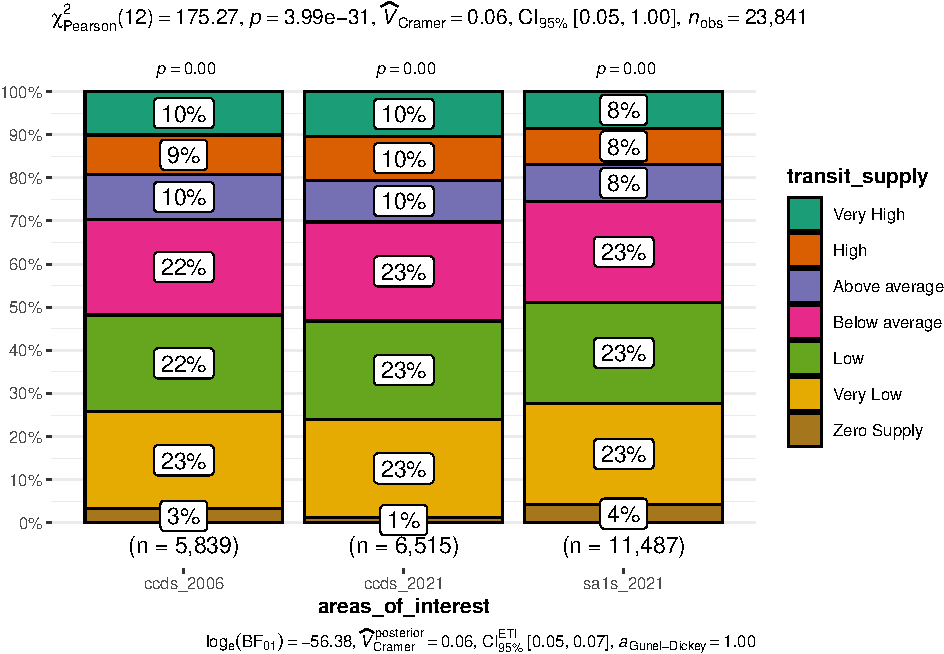
\includegraphics{Leveraging_GTFS_to_assess_transit_supply_Transport_Geography_files/figure-latex/Greater_Melbourne_SA1_2021_table-1.pdf}
\caption{Greater Melbourne: distribution of supply index scores, 2006
CCDs, 2021 CCDs and 2021 SA1s}
\end{figure}

A smaller proportion of CCDs have Zero Supply in 2021 than 2006,
suggesting that transit now covers more of city. However, Greater
Melbourne now covers a larger spatial area than it did in 2006, and most
of the new additions appear to have Zero or Very Low transit supply.
Hence, looking at the overall picture for 2021 the proportion of SA1s
with Zero Supply or with supply below the average is larger than was the
case for CCDs in 2006.

\begin{figure}
\centering
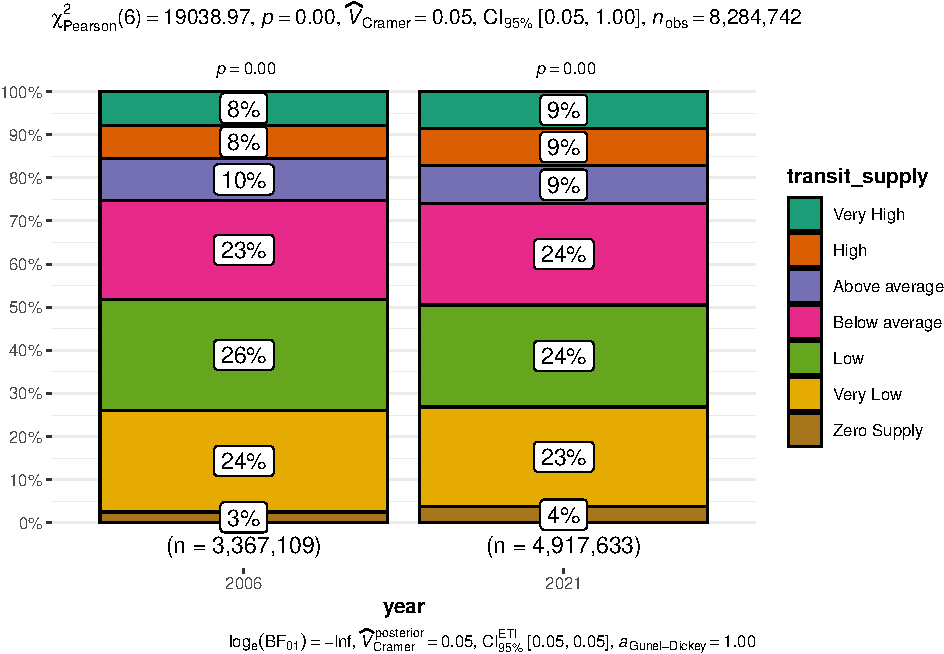
\includegraphics{Leveraging_GTFS_to_assess_transit_supply_Transport_Geography_files/figure-latex/Greater_Melbourne_population_figure-1.pdf}
\caption{Greater Melbourne: population distribution of supply index
scores. Sources: 2006 values (Currie2010), 2021 values (authors)}
\end{figure}

Table \ref{tab:Greater_Melbourne_SA1_2021_table} and Figure
\ref{fig:Greater_Melbourne_population_figure} show that the proportion
of the population in zones with Zero Supply was higher in 2021 than in
2006. but a slightly larger share of the population are in zones with SI
scores above the average.

\subsubsection{2021 Social needs}\label{social-needs}

Figure \ref{fig:Greater_Melbourne_2021_social_needs} shows the
distribution of categories of social need index scores across Greater
Melbourne for 2021. This figure is analogous to the 2006 value from
\citet{currie2010identifying} shown in Figure \ref{fig:Currie_map_needs}
although, as discussed in the methodology section above, it was not
possible to exactly replicate the \citet{currie2010identifying} approach
due to changes in the way census results are reported.

\begin{figure}
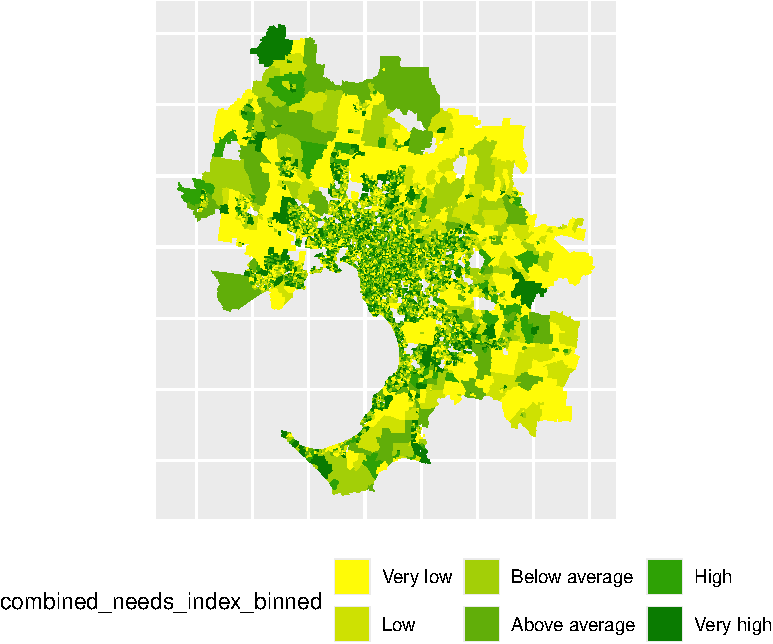
\includegraphics[width=0.9\linewidth]{Leveraging_GTFS_to_assess_transit_supply_Transport_Geography_files/figure-latex/Greater_Melbourne_2021_social_needs-1} \caption{Distribution of categories of composite social need index scores, with 2006 Melbourne boundary shown in black. Source: authors analysis of ABS data}\label{fig:Greater_Melbourne_2021_social_needs}
\end{figure}

Figure \ref{fig:Greater_Melbourne_2021_social_needs} appears to indicate
that there is no clear spatial pattern to the distribution of the
categories of the composite need index scores. This appears to contrast
to trend, albeit with some exceptions, towards very high social needs
scores in outer areas identified by \citet{currie2010identifying}
(Figure \ref{fig:Currie_map_needs}). This may, however, be an artifact
of either the differences in the composite needs scores used in this
analysis (due to the lack of data to assess relative needs) compared to
the \citet{currie2010identifying} analysis. As well, the 2021 census SA1
zones generally appear to smalller than the 2006 Census Collection
Districts (CCDs) used in \citet{currie2010identifying}, especially in
outer areas. This will be associated with the growth of Greater
Melbourne's population and spatial dispersment, with many of the large
outer `Very High' CCDs shown in the 2006 map now split into many more
SA1 zones.

\subsubsection{Needs-gap analysis}\label{needs-gap-analysis}

\subsection{Variation in spatial patterns across Australian
cities}\label{variation-in-spatial-patterns-across-australian-cities}

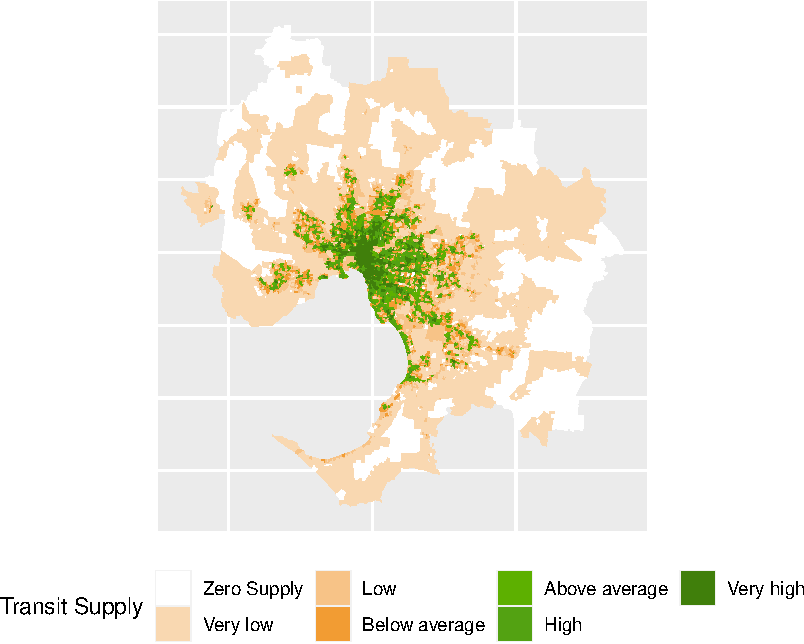
\includegraphics{Leveraging_GTFS_to_assess_transit_supply_Transport_Geography_files/figure-latex/Australian_cities_2021-1.pdf}
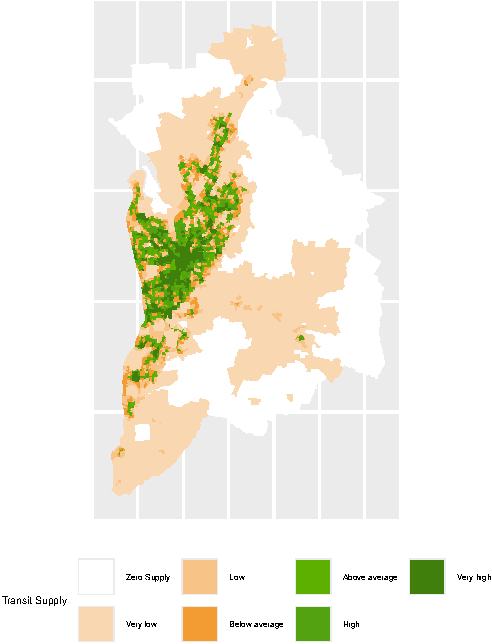
\includegraphics{Leveraging_GTFS_to_assess_transit_supply_Transport_Geography_files/figure-latex/Australian_cities_2021-2.pdf}
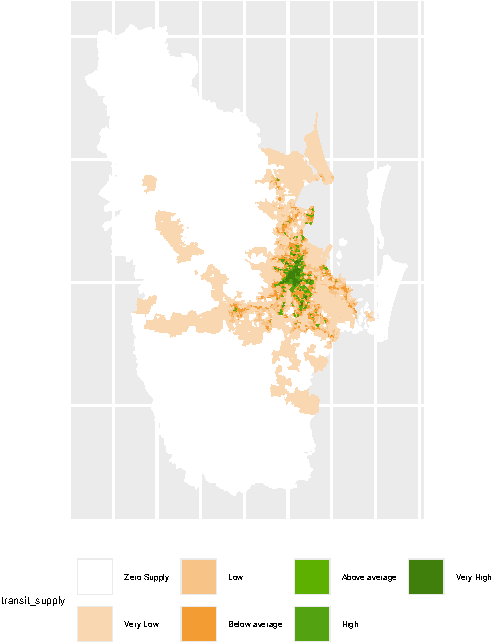
\includegraphics{Leveraging_GTFS_to_assess_transit_supply_Transport_Geography_files/figure-latex/Australian_cities_2021-3.pdf}
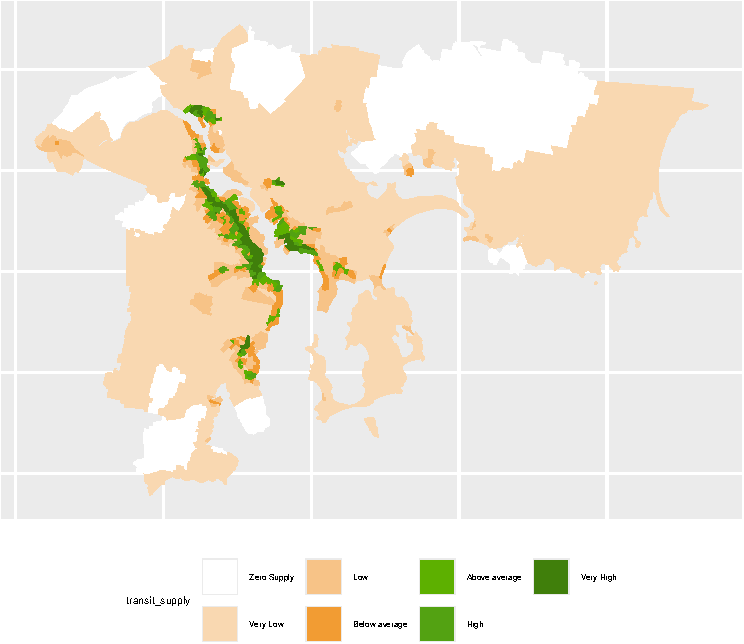
\includegraphics{Leveraging_GTFS_to_assess_transit_supply_Transport_Geography_files/figure-latex/Australian_cities_2021-4.pdf}
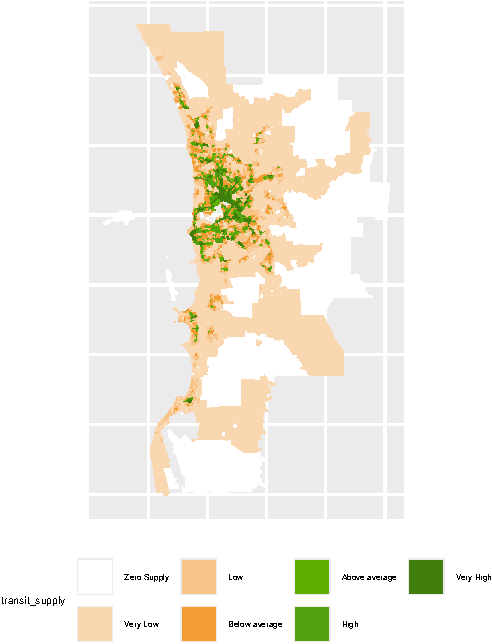
\includegraphics{Leveraging_GTFS_to_assess_transit_supply_Transport_Geography_files/figure-latex/Australian_cities_2021-5.pdf}

Figure \ref{fig:Australian_cities_2021} shows SI values for the week
starting on the day of the 2021 census for all Australian Capital Cities
except Greater Sydney, for which the SI values are calculated for the
week starting .

\section{Discussion}\label{discussion}

\subsection{Limitations}\label{limitations}

\subsection{Directions for furture
research}\label{directions-for-furture-research}

\section{Conclusions}\label{conclusions}

\section*{References}\label{references}
\addcontentsline{toc}{section}{References}

\renewcommand\refname{Appendix A - GCCSA maps by SA1}
\bibliography{References.bib, packages.bib}


\end{document}
